%=========================================================

% Here you can choose to compile with or without solutions.
% However, this definition is ignored if you use any
% command from the `Makefile`.
\providecommand{\withSol}{\iftrue}

%=========================================================

\documentclass
[twoside,english,colorbacktitle,accentcolor=tud9c]
{tudexercise}

\usepackage[T1]{fontenc}
\usepackage[latin9]{inputenc}
\usepackage{amstext}
\usepackage{amsmath}
\usepackage{graphicx}
\usepackage{setspace}
\usepackage{multicol}
\usepackage{mathtools}
\usepackage{dsfont}
\usepackage{units}
\usepackage{subfigure}
\usepackage{color}
\usepackage{booktabs}
\usepackage{fancyref}
\usepackage[ngerman,english]{babel}
\usepackage{color}

%=========================================================

\def\homework{2}
\def\homeworkVer{1}
\def\homeworkSolVer{1}

%=========================================================

\ifcsname withSol\endcsname\else
  \expandafter\let\csname withSol\expandafter\endcsname
                  \csname iffalse\endcsname
\fi

\withSol
	\usepackage[solutions]{iasHomework}
\else
	\usepackage{iasHomework}
\fi

%=========================================================

\hwtitle{Robot Learning}
{Winter Semester 2016}
{Prof. Dr. J. Peters, F. Veiga, S. Parisi}

\begin{document}

%=========================================================

\maketitle

\begin{examheader}
	\textmb{Robot Learning - Homework \arabic{section}}
	\examheaderdefault 
\end{examheader} 

\deadline{Thursday, 12 January 2017 (before the lecture)}

%=========================================================

\exercise{Model Learning}
The new and improved Spinbot 2000 is a multi-purpose robot platform.
It is made of a kinematic chain consisting of a linear axis $q_{1}$, a rotational axis $q_{2}$ and another linear axis $q_{3}$, as shown in the figure below.
These three joints are actuated with forces and torques of $u_{1}$, $u_{2}$, and $u_{3}$.
Different end effectors, including a gripper or a table tennis racket, can be mounted on the end of the robot, indicated by the letter $E$.
Thanks to Spinbot's patented SuperLight technology, the robot's mass is distributed according to one point mass of $m_{1}$ at the second joint and another point mass of $m_{2}$ at the end of the robot $E$.

%\includegraphics[width=0.5\textwidth]{fig/spinbot.eps}
\colorbox{yellow}{Your graphic could be here. It just wasn't included.}

The inverse dynamics model of the Spinbot is given as
\begin{align*}
u_{1} &= (m_{1}+m_{2})(\ddot{q}_{1}+g),\\
u_{2} &= m_{2}(2\dot{q}_{3}\dot{q}_{2}q_{3}+q_{3}^{2}\ddot{q}_{2}),\\
u_{3} &= m_{2}(\ddot{q}_{3}-q_{3}\dot{q}_{2}^{2}).
\end{align*}
We now collected 100 samples from the robot while using a PD controller with gravity compensation at a rate of 500Hz.
The collected data (see \texttt{spinbotdata.txt}) is organized as follows\\
\begin{tabular}{| l || c | c | c | l  }
  \hline
   & $t_1$ & $t_2$ & $t_3$ & \ldots\\
  \hline
  \hline
  $q_{1}[m]$ &  &  &  & \\
  \hline
  $q_{2}[rad]$ &  &  &  & \\
  \hline
  $q_{3}[m]$ &  &  &  & \\
  \hline
  \ldots &  &  &  &  \\
  \hline
  $\ddot{q}_{3}[m/s^{2}]$ &  &  &  & \\
  \hline
  $u_{1}[N]$ &  &  &  & \\
  \hline
  $u_{2}[Nm]$ &  &  &  & \\
  \hline
  $u_{3}[N]$ &  &  &  & \\
  \hline
\end{tabular}

Given this data, you now want to learn the inverse dynamics of the robot in order to use a model-based controller.
The inverse dynamics of the system will be modeled as $\vec{u}=\vec{\phi}(\vec{q},\dot{\vec{q}},\ddot{\vec{q}})^{\T}\vec{\theta}$, where $\vec{\phi}(\vec{q},\dot{\vec{q}},\ddot{\vec{q}})$ are features and $\vec{\theta}$ are the parameters.

\begin{questions}

%----------------------------------------------

\begin{question}{Problem Statement}{1}
What kind of machine learning problem is learning an inverse dynamics model?

\begin{answer}
	It is a supervised learning problem. The reason being that it tries to map input to output on labelled data.
\end{answer}

\end{question}

%----------------------------------------------


\begin{question}{Assumptions}{5}
Which standard assumption has been violated by taking the data from trajectories?

\begin{answer}
	%TODO Wirkt zu einfach. Nachprüfen.
	We are not learning a function with this. This is a problem as there can be many solutions to one problem resulting in difficulties when learning (using the mean is not useful as the mean of two solutions is itself far off).
\end{answer}

\end{question}

%----------------------------------------------


\begin{question}{Features and Parameters}{4}
Assuming that the gravity $g$ is unknown, what are the feature matrix $\vec{\phi}$ and the corresponding parameter vector $\vec{\theta}$ for $\vec{u}=[u_{1},u_{2},u_{3}]^{\T}$?
(Hint: you do not need to use the data at this point)

\begin{answer}
$$\vec{\phi}=
\begin{bmatrix}
\ddot{q}_1 & 0 & 0  \\
\ddot{q}_1 & 2\dot{q}_3\dot{q}_2q_3+q_3^2\ddot{q}_2 & \ddot{q}_3-q_3\dot{q}_2^2  \\
1 & 0 & 0 
\end{bmatrix}$$
$$
\vec{\theta}= 
\begin{bmatrix} 
	m_{1} & m_{2} & g \cdot (m_{1}+m_{2})\\
\end{bmatrix}$$
\end{answer}
\end{question}


%----------------------------------------------


\begin{question}{Learning the Parameters}{2}
You want to compute the parameters $\vec{\theta}$ minimizing the squared error between the estimated forces/torques and the actual forces/torques.
Write down the matrix equation that you would use to compute the parameters. For each matrix in the equation, write down its size.\\
Then, compute the least-squares estimate of the parameters $\vec{\theta}$ from the data and report the learned values.

\begin{answer}

$\theta = (\phi\phi^{T})^{-1}\phi Y$ \\
$\theta \in \mathbb{R}^{3\times1},$\\
$\phi \in \mathbb{R}^{3\times300},$\\
$\phi^T \in \mathbb{R}^{300\times3},$\\
$Y \in \mathbb{R}^{300\times1}$\\
$\vec{\theta}= 
\begin{bmatrix} 
	-0.07297389 \\
	1.6496578 \\
	15.09510
\end{bmatrix}$
\end{answer}

\end{question}

%----------------------------------------------


\begin{question}{Recovering Model Information}{4}
	Can you recover the mass properties $m_{1}$ and $m_{2}$ from your learned parameters? Has the robot learned a plausible inverse dynamics model? Explain your answers.
	
\begin{answer}
Unfortunately, we cannot recover the mass properties from our learned parameter, since our first parameter, which denoted $m_1$, is negative. From this we deduct, that our learned parameters are not the ones we considered them to be. So the model didn't learn a plausible inverse dynamics model, but some values for the parameters so that the joints were approximated.
\end{answer}
\end{question}

%----------------------------------------------


\begin{question}{Model Evaluation}{7}
Plot the forces and torques predicted by your model over time, as well as those recorded in the data and comment the results. Is the model accuracy acceptable? If not, how would improve your model? Use one figure per joint.

\begin{answer}
	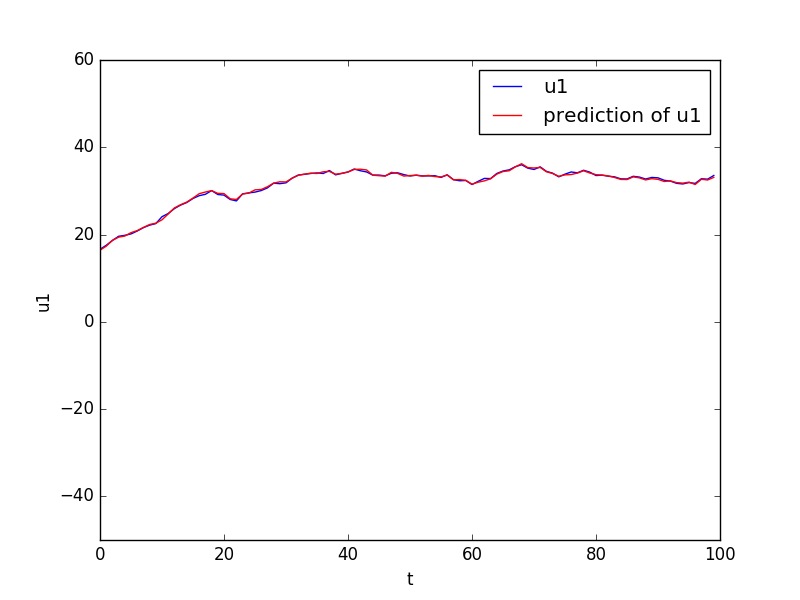
\includegraphics[width=87mm]{first_joint.png}
	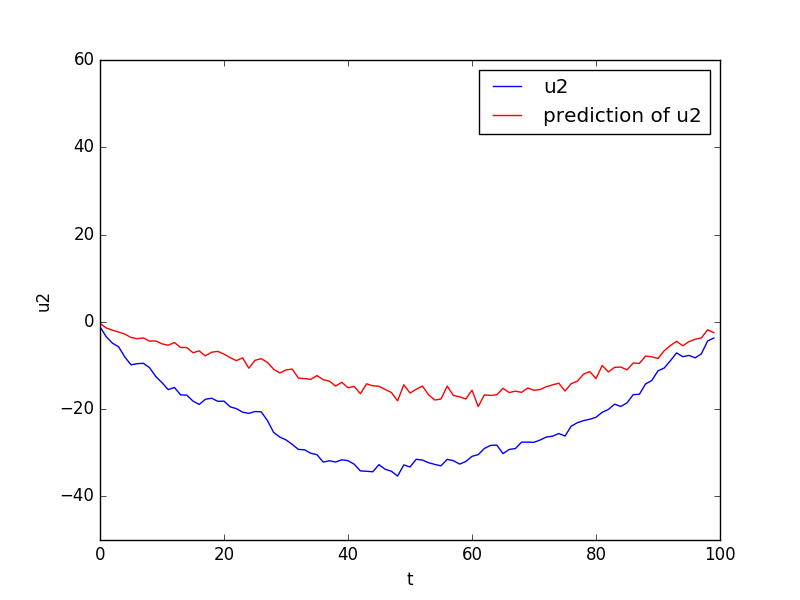
\includegraphics[width=87mm]{second_joint.png}
	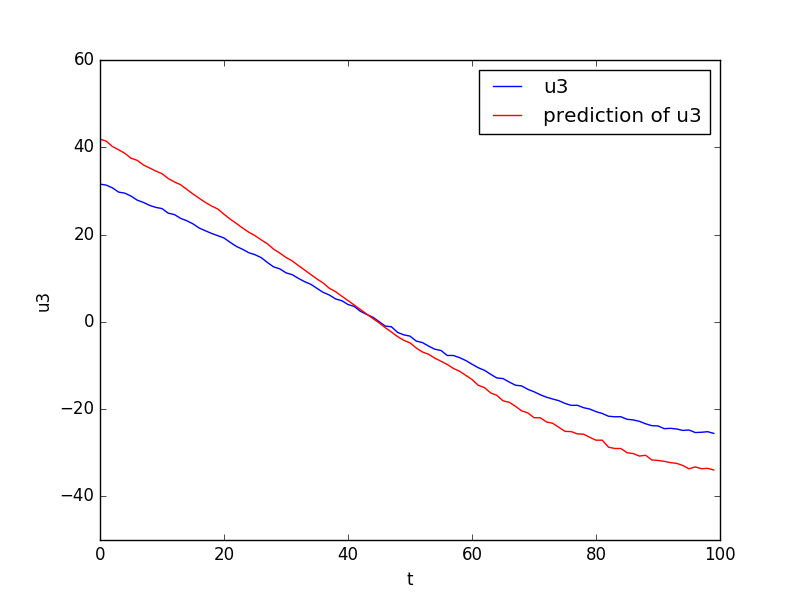
\includegraphics[width=87mm]{third_joint.png}\\
	
	The prediction for the first joint is very precise.\\
	The second plot shows that the prediction for the second joint at least has the same trend as the real values, but differ especially at around half of the time.\\
	The predictions of the third joint differ at the beginning and the end the most, and are better at around half of the time. 
	All in all the models accuracy is not acceptable, since the calculated values for the second and third joints differ to much at some points.\\
	
	To improve the model, it would be better if we could integrate the gravity constant directly into the feature matrix, instead of learning it as a parameter, since it is a well known constant. Moreover, a larger dataset could be an advantage.

\end{answer}

\end{question}

%----------------------------------------------


\begin{question}[bonus]{Models for Control}{4}
Name and describe three different ways to use learned models in control laws or for generating control laws.

\begin{answer}
We can use \textbf{Controller Falsification} which uses our model to test random Control Laws and outputs the first one that does not fail.\\
We can also use it to \textbf{optimize our control law} by generating control laws and comparing them to our current best control law. \\
We can also use our learned model to \textbf{generate a policy} that simplifies our control.
\end{answer}

\end{question}

%----------------------------------------------

\end{questions}


\newif\ifvimbug
\vimbugfalse

\ifvimbug
\begin{document}
\fi

\exercise{Trajectory Generation with Dynamical Systems}
In this exercise we will use the Dynamic Motor Primitives (DMPs), described by the following dynamical system,
%
\begin{align}
    \ddot{y}&=\tau^2(\alpha(\beta(g-y)-(\dot{y}/\tau))+f_w(z)), \label{eq:dmp} \\
    \dot{z}&=-\tau\alpha_zz, \label{eq:dmp_phase}
\end{align}
%
where $y$ is the state of the system, $\dot{y}$ and $\ddot{y}$ are the first and second time derivatives, respectively. The attractor's goal is denoted by $g$ and the forcing function by $f_w$. The parameters $\alpha$ and $\beta$ control the spring-damper system. The phase variable is denoted by $z$ and the temporal scaling coefficient by $\tau$. The forcing function $f_w$ is given by
%
\begin{equation}
    f_w(z)=\frac{\sum_{i=0}^{K}\phi_{i}(z)w_{i}z}{\sum_{j=0}^{K}\phi_{j}(z)}=\vec{\psi}(z)^{T}\vec{w},
    \quad \textrm{with}\quad \psi_i(z) = \frac{\phi_i(z)z}{\sum_{j=1}^K\phi_j(z)},
\end{equation}
%
where the basis functions $\phi_i(z)$ are Gaussian basis given by
%
\begin{equation}
    \phi_i(z) = \exp(-0.5(z-c_i)^2/h_i),
\end{equation}
where the centers $c$ are equally distributed in the phase $z$, and the width $h$ is an open parameter. For the programming exercises a basic environment of a double link pendulum is provided, as well as the computation of the $\vec{\psi}_i(z)$.


\begin{questions}

%----------------------------------------------

\begin{question}{Similarities to a PD controller}{2}
Transform Equation~\eqref{eq:dmp} to have a similar structure to a PD-controller,
%
\begin{equation}
    \ddot{y}_z = K_P ( y^{des}_z - y_z ) + K_D ( \dot{y}_z^{des} - \dot{y}_z ) +
    u_{ff}
\end{equation}
%
and write down how the following quantities $K_p, K_d, y^{des}_z$ and $\dot{y}_z^{des}$ look like in terms of the DMP parameters. Do not expand the forcing function $f_w(z)$ at your solutions.

\begin{answer}
\begin{align*}
	\ddot{y}_{z} & = \tau^2\alpha\beta\cdot (g-y) + \frac{\alpha}{\tau}\cdot(0-\dot{y}) + \tau^2 f_{w}(z)\\
	K_p & = \tau^2\alpha\beta\\
	K_d & = \frac{\alpha}{\tau}\\
	y_{z}^{des} & = g\\
	\dot{y}_{z}^{des} & = 0\\
\end{align*}
\end{answer}

\end{question}

%----------------------------------------------

\begin{question}{Stability}{2}
Show why the DMPs are stable when $t\to\infty$ and what would the equilibrium point be.

\begin{answer}\end{answer}

\end{question}

%----------------------------------------------

\begin{question}{Double Pendulum - Training}{12}
Implement the DMPs and test them on the double pendulum environment.
In order to train the DMPs you have to solve Equation~\eqref{eq:dmp} on the forcing function. Before starting the execution, set the goal $g$ position to be the same as in the demonstration. Then, set the parameters to $\alpha=25, \beta=6.25, \alpha_z=3/T, \tau=1$. Use $N=50$ basis functions, equally distributed in $z$.  Use the learned DMPs to control the robot and plot in the same figure both the demonstrated trajectory and the reproduction from the DMPs.
You need to implement the DMP-based controller (\texttt{dmpCtl.py}) and the training function for the controller parameters (\texttt{dmpTrain.py}). To plot your results you can use \texttt{dmpComparison.py}. Refer to \texttt{example.py} to see how to call it. Attach a snippet of your code.

\begin{answer}\end{answer}

\end{question}



%----------------------------------------------

\begin{question}{Double Pendulum - Conditioning on the Final Position}{3}
Using the trained DMPs from the previous question, simulate the system with different goal positions: first with $q_{t=\mathrm{end}} = \{0, 0.2\}$ and then with $q_{t=\mathrm{end}} = \{0.8, 0.5\}$. Generate one figure per DoF. In each figure, plot the demonstrated trajectory and the reproduced trajectories with different goal positions.
How do you interpret the result? 

\begin{answer}\end{answer}


\end{question}

%----------------------------------------------

\begin{question}{Double Pendulum - Temporal Modulation}{3}
Using the trained DMPs from the previous question, simulate the system with different temporal scaling factors $\tau=\{0.5, 1.5\}$. Generate one figure per DoF and explain the result.

\begin{answer}\end{answer}


\end{question}

%----------------------------------------------

\begin{question}[bonus]{Probabilistic Movement Primitives - Radial Basis Function}{3}
We now want to use ProMPs. Before we train them, we need to define some basis functions. We decide to use $N = 30$ radial basis functions (RBFs) with centers uniformly distributed in the time interval $[0-2b,T+2b]$, where $T$ is the end time of the demonstrations.
The bandwidth of the Gaussian basis (std) is set to $b=0.2$. 
Implement these basis functions in \texttt{getProMPBasis.py}. 
Do not forget to normalize the basis such at every time-point they sum-up to one! Attach a plot showing the basis functions in time and a snippet of your code. 

\begin{answer}\end{answer}
\end{question}

%----------------------------------------------

\begin{question}[bonus]{Probabilistic Movement Primitives - Training}{7}
In this exercise you will train the ProMPs using the imitation learning data from \texttt{getImitationData.py} and the RBFs defined in the previous question. Modify the \texttt{proMP.py} in order to estimate weight vectors $w_i$ reproducing the different demonstrations. Then, fit a Gaussian using all the weight vectors. Generate a plot showing the desired trajectory distribution in time (mean and std) as well as the trajectories used for imitation. Attach a snippet of your code.

\begin{answer}\end{answer}

\end{question}

%----------------------------------------------

\begin{question}[bonus]{Probabilistic Movement Primitives - Number of Basis Functions}{2}
Evaluate the effects of using a reduced number of RBFs. Generate two plots showing the desired trajectory distribution and the trajectories used for imitation as in the previous exercise, but this time use $N=20$ and $N=10$ basis functions. Briefly analyze your results.

\begin{answer}\end{answer}

\end{question}

%----------------------------------------------


\begin{question}[bonus]{Probabilistic Movement Primitives - Conditioning}{4}
Using Gaussian conditioning calculate the new distribution over the weight vectors $w_i$ such as the trajectory has a via point at position $y^*=3$ at time $t_\textrm{cond}=1150$ with variance $\Sigma_{y^*}=0.0002$.
Assuming that the probability over the weights is given by $\mathcal{N}(\vec w|\vec \mu_w,\vec \Sigma_w)$ and the probability of being to that position is given by $\mathcal{N}(y^*|\vec \Phi \vec w, \Sigma_{y^*} )$, show how the new distribution over $\vec w$ is computed (how does the mean and variance look like)?
\\
Then, in a single plot, show the previous distribution (learned from imitation) and the new distribution (after conditioning). Additionally, sample $K=10$ random weight vectors from the ProMP, compute the trajectories and plot them in the same plot. Analyze briefly your results and attach a snippet of your code.

\begin{answer}\end{answer}

\end{question}

\end{questions}


%=========================================================

\end{document}
